\documentclass[tikz, border=10pt]{standalone}
\usepackage{tikz}
\usetikzlibrary{positioning, arrows.meta, backgrounds}

\tikzstyle{n} = [circle, draw, minimum size=0.8cm, align=center]

\begin{document}
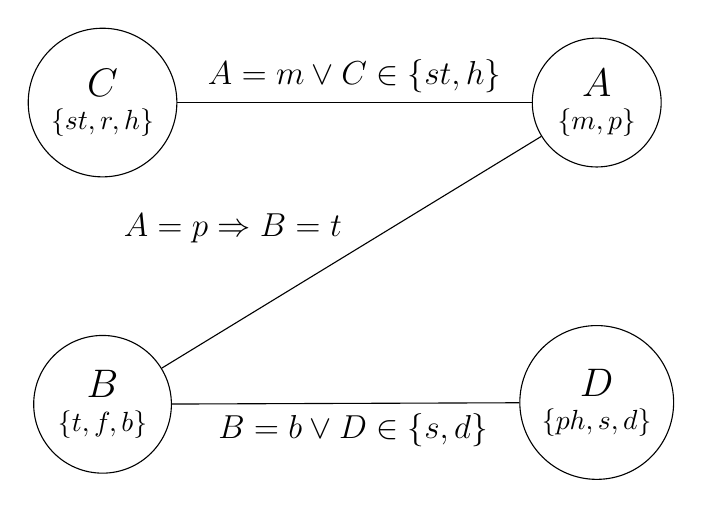
\begin{tikzpicture}[node distance=2cm and 4.5cm]

    \node[n] (C) {
        \Large $C$ \\ $\{st, r, h\}$
    };
    \node[n, right=of C] (A) {
        \Large $A$ \\ $\{m, p\}$
    };
    \node[n, below=of C] (B) {
        \Large $B$ \\ $\{t, f, b\}$
    };
    \node[n, below=of A] (D) {
        \Large $D$ \\ $\{ph, s, d\}$
    };

    % Define edges with labels
    \path[-]
        (A) edge node[above] {\large $A = m \lor C \in \{st, h\}$} (C)
        (B) edge node[above left] {\large $A = p \Rightarrow B = t$} (A)
        (B) edge node[below] {\hspace{2pt} \large $B = b \lor D \in \{s, d\}$} (D);

\end{tikzpicture}
\end{document}